In the framework of hand prosthetics, one usually operates the
distinction between passive and active hand prostheses. As the name
suggests, an active hand prosthesis (AHP) is a hand prosthesis which
can be voluntarily actuated, to some degree, by the patient wearing
it. Besides being cheap, visually appealing, lightweight and
long-running, the ideal AHP is highly dexterous and easily
controlled. Sensorial feedback completes the picture, making the
prosthesis a sensible replacement of the lost hand.

At the time of writing, however, the state-of-the-art of AHPs is far
from this. The best known commercially available AHPs are Otto Bock's
SensorHand \cite{sensorhand} and Touch Bionics's i-LIMB
\cite{ilimb}. The SensorHand is a classical one-DOF ``claw'',
proportionally controlled typically by one or two electromyography
electrodes; the i-Limb has five independently moving fingers plus a
passively opposable thumb, but only uses two electrodes and, as far as
one can understand, offers no fine control over single fingers or over
the required amount of force. Nevertheless, one can see a definite
move forward as far as the mechatronics is concerned --- a drive which
mainly comes from miniaturised electronics and humanoid robotics;
examples of this are, e.g., the DLR prosthetic hand (\cite{Hua2006}
--- see Figure \ref{fig:DLRHandII}) and the the CyberHand
\cite{cyberhand}.

\begin{figure}
  \begin{tabular}{cc}
    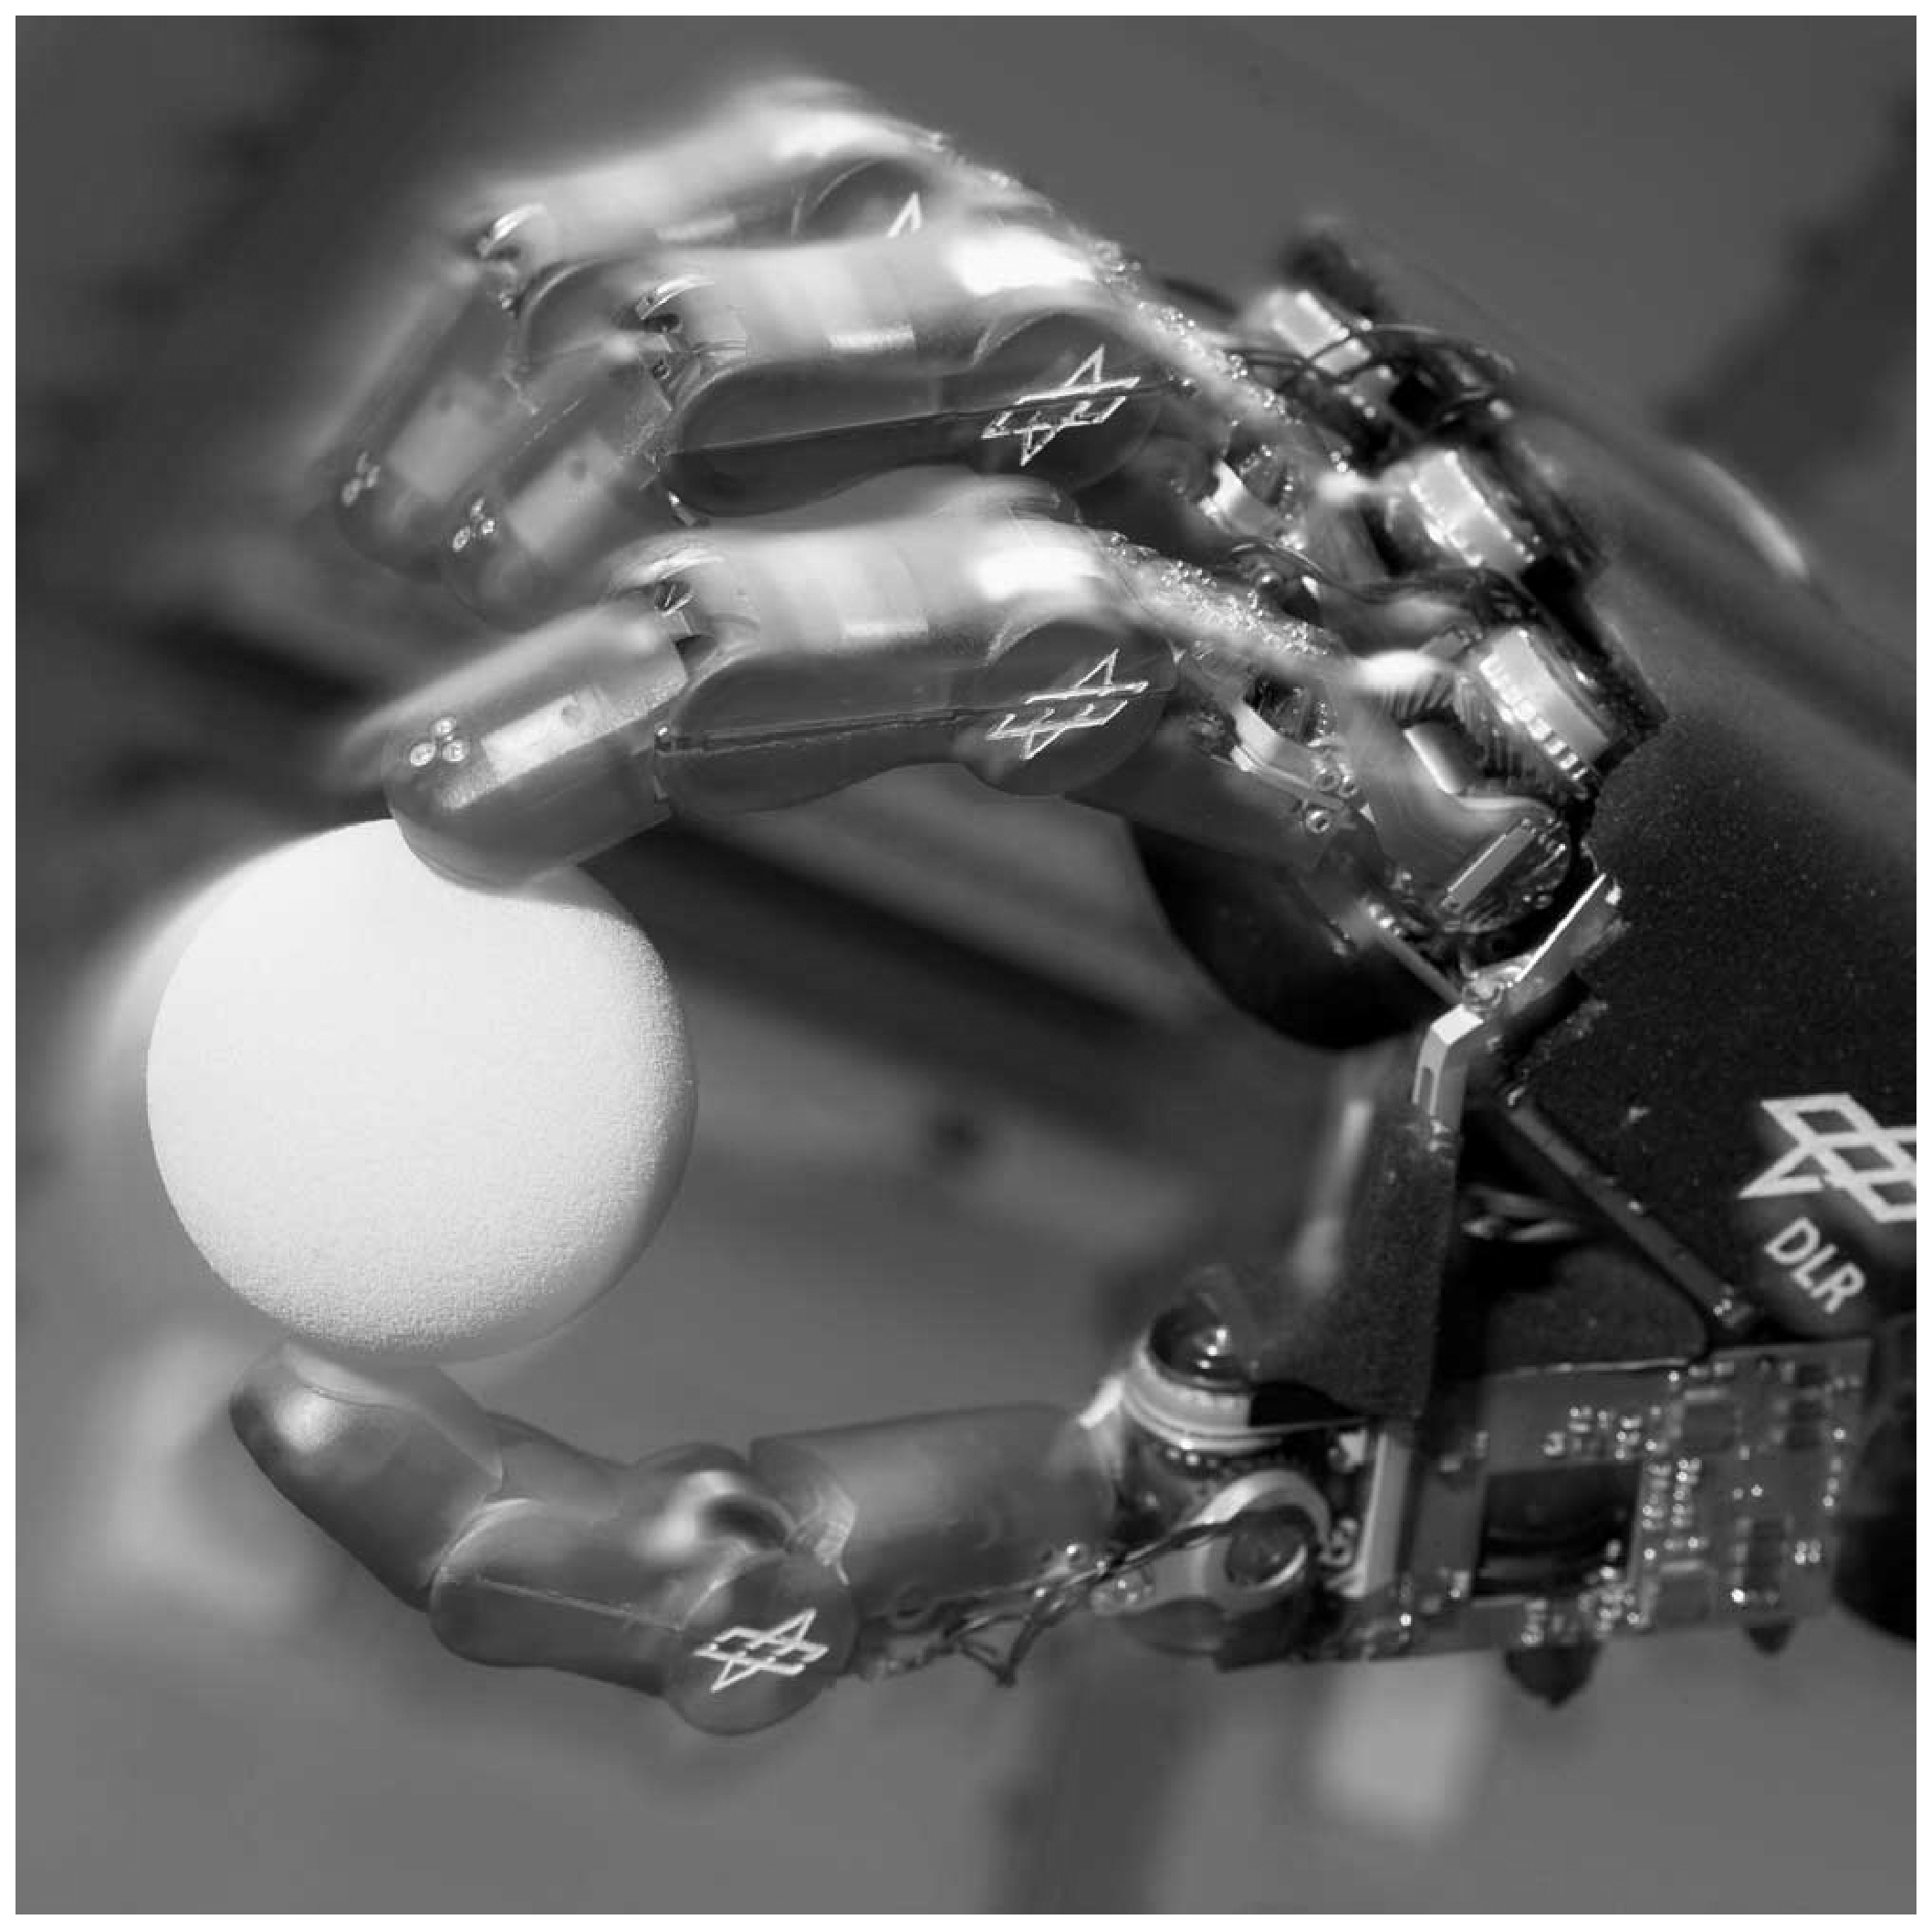
\includegraphics[height=0.12\textheight]{figs/DLRHand-Ball-comp.eps} &
    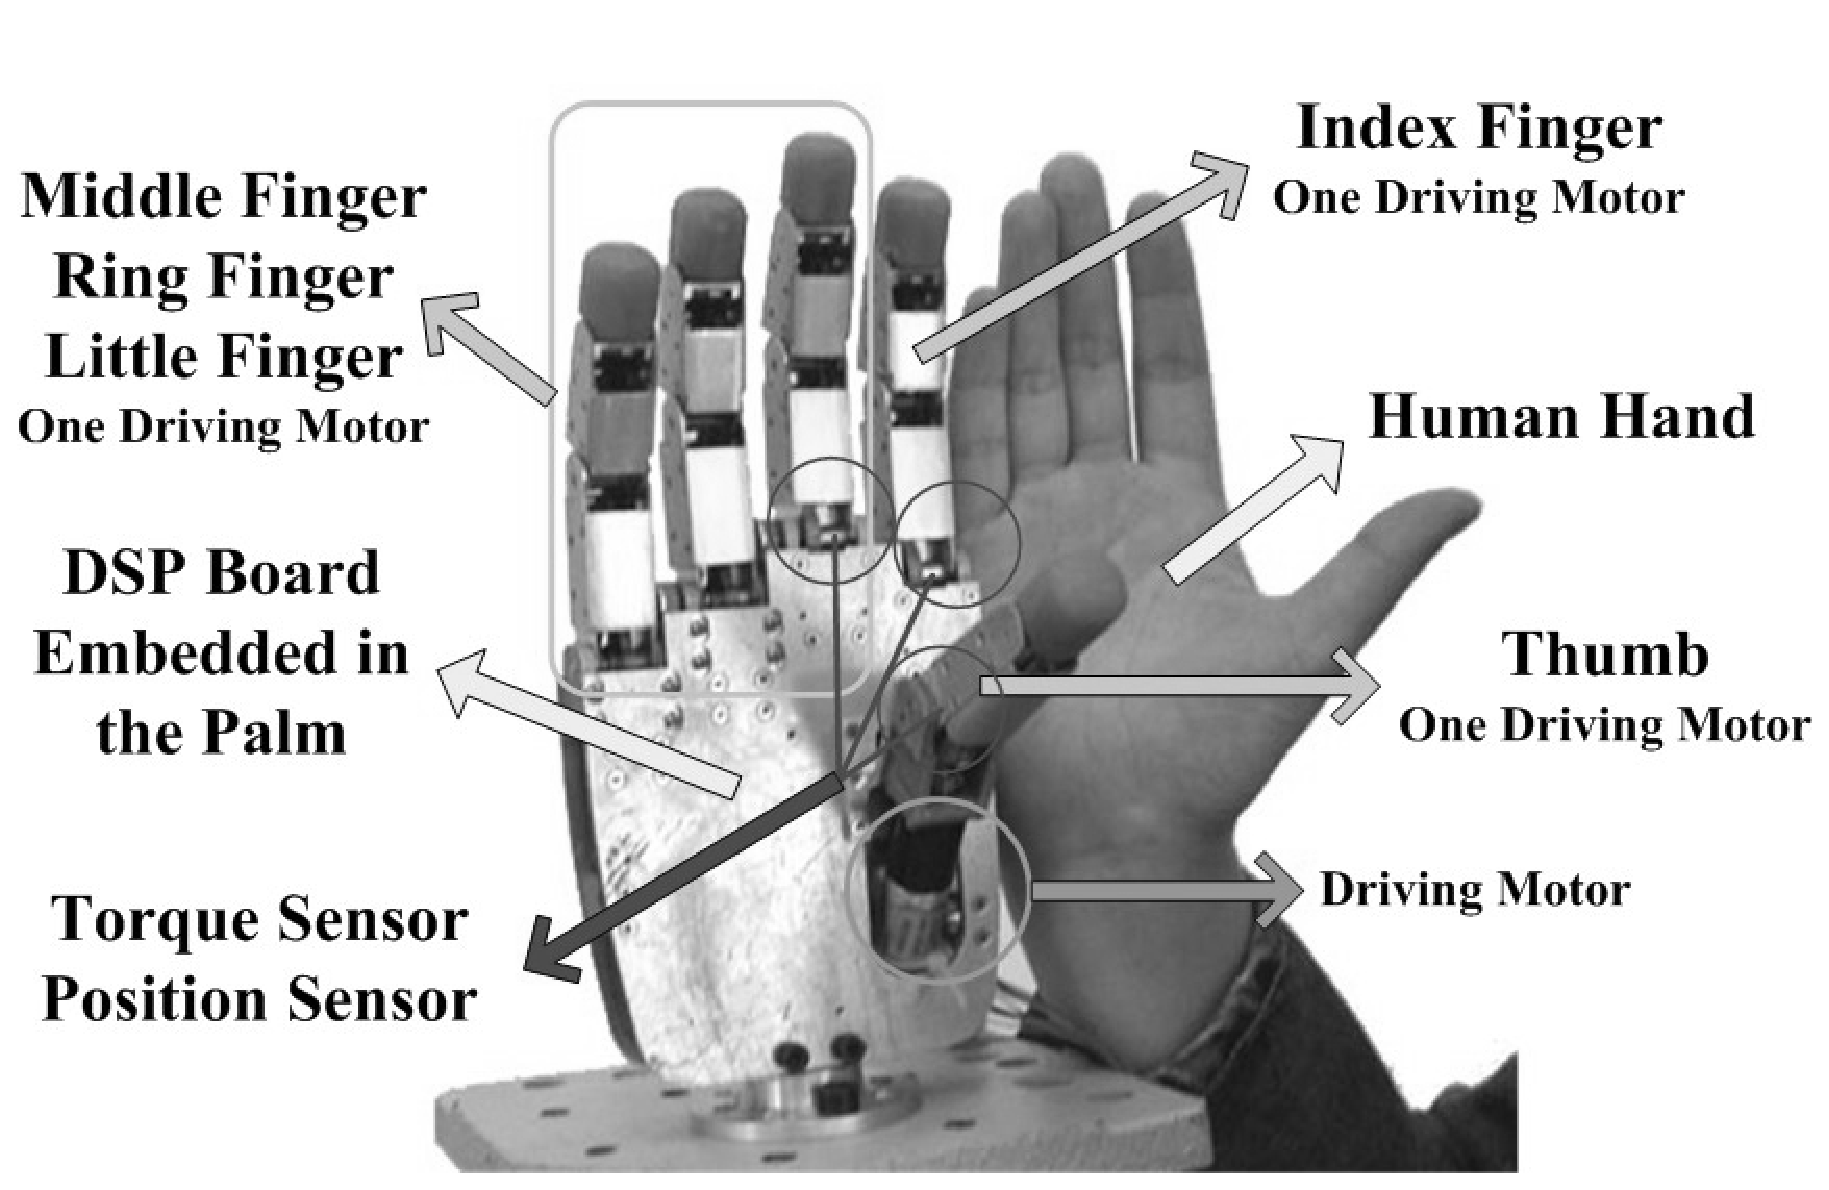
\includegraphics[height=0.12\textheight]{figs/DLR-Prothese.eps}
  \end{tabular}
  \caption{(left) The DLR Hand II. (right) The DLR prosthetic hand.}
  \label{fig:DLRHandII}
\end{figure}

It seems then that the problem of \emph{control} by the patient is
going to be a major issue in the next years. As the prosthetic hand
becomes more and more flexible, how is the patient supposed to
precisely command the prosthesis what to do? Operating a hand requires
a fine control, possibly down to the level of the single fingers:
first of all, presented with a certain task such as turning a door
handle or grabbing a car key, the patient must be able to enforce the
correct grasping type; this involves the activation of some joints
only, and in particular positions. Secondly, the amount of force
involved in the grasp must be controlled, so that it is possible to
grab, e.g., both a hammer without letting it slip and an egg without
breaking it. Thirdly, feedback to the patient is paramount.

As far as the feed-forward path is concerned, that is, sending
commands to the prosthesis, two types of interfaces between the
patient and the prosthesis have been developed or are being studied:
\emph{invasive} and \emph{non-invasive}. The former gather control
signals directly from the user's nervous system, either via brain
implants or surgical use of electrodes. Quite obviously, invasive
interfaces are supposed to deliver a high signal quality, since the
signals can be gathered exactly in the right spots; but they involve
surgery and all related sterility (and psychological) issues. On the
other hand, non-invasive interfaces are easier to handle and maintain,
but require a much better signal conditioning, since they usually work
with surface (skin) signals or vision and gaze tracking.

In the context of non-invasive interfaces for controlling mechanical
hands, a concrete possibility arises from \emph{forearm surface
electromyography} (EMG), a technique by which muscle activation
potentials are gathered by electrodes placed on the patient's forearm
skin; these potentials can be used to track which muscles the patient
is willing to activate, and with what force. Surface EMG is therefore,
in principle, a cheap and easy way of detecting what the patient wants
the prosthesis to do.

Using the EMG to feed-forward control an AHP requires adaptivity,
accuracy and speed: each single patient must be able to control the
prosthesis accurately in real time. These characteristics belong to
\emph{machine learning}, which has in fact already been applied to EMG
in the classification of isotonic hand postures of healthy subjects
\cite{ekvall,smagt}; but so far, no indication about the amount of
force involved in the grasping act is detected.

In this paper we go one step beyond by applying machine learning
techniques to the forearm EMG signal generated by a healthy subject in
controlled conditions. Three machine learning approaches have been compared:
(a) a simple feed-forward neural network with one hidden layer,
(b) a Support Vector Machine with radial basis function kernel
\cite{BGV92}, and (c) Locally Weighted Projection Regression
\cite{lwpr}. Our analysis benefits from a simple but effective procedure
for selecting a subset of the samples on-the-fly, called \emph{Online
Uniformisation} (OU); and in the end it shows that there is no clear
winner among the tested approaches, but that, as a whole, the idea is
viable. The resulting system, in fact, guesses \emph{both} $(a)$ what
kind of grasp the subject is applying, and $(b)$ how much force the
subject is exerting. The system attains remarkable accuracy: the type
of grasp can be reconstructed with an average accuracy of $89.67\% \pm
1.53\%$, and the applied force can be predicted with an average
percentage error of $7.89\% \pm 0.09\%$, meaning $4.5$N over a range
of about $57$N.

Lastly, the system has been really tested on-line on the DLR-II Hand
(see \cite{ButFisGre2004}), which is a dexterous, multifingered
robotic hand, although not a prosthetic one. The system was able to
control it in impedence, to the point of grasping an egg without
breaking it, and then to actually break it, when the subject would
tighten the grip.

All in all, the results in this paper lay the basis for the
feed-forward control of the next generation AHPs. The last big step is
to check whether an amputee's forearm still contains enough muscular
potential activity to obtain the same results. This is the main
subject of future research, along with feedback, to better close the
sensorimotor loop between the patient and the prosthesis.

The paper is structured as follows: after a brief review of relevant
literature, we describe in detail the experiment and the methods used
to tackle it (Section \ref{sec:m&ms}); then we show and comment on the
experimental results (Section \ref{sec:exp}); lastly, discussion and
conclusions are presented.
